% !TEX root = ../main.tex
\subsection*{Brutal Criticals} \label{ssec::brutalcriticals}

Presented here are optional rules that expand the scope of critical hits.
Introducing a series of critical hit charts that vary based on the damage type of the attack, this module adds an additional element of uncertainty, suspense, and surprise to combat.

\subsubsection{Revisions to Critical Hits}
    \begin{itemize}
        \item When you land a critical hit on a creature, roll the damage dice twice and add them together as normal.
        Then, roll a d20 and use the corresponding result on the critical hit chart determined by the damage type of your attack.
        \item When you score a critical hit with an attack that does two or more types of damage, choose one of those damage types and roll on that critical chart.
        \item Traits and feats like Savage Attacks and Brutal Critical continue to work as written.
    \end{itemize}

\begin{figure}[t]
    \centering
    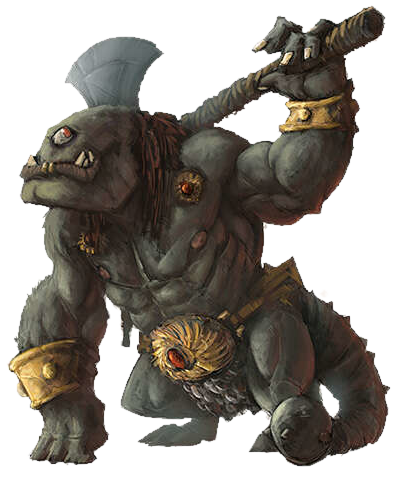
\includegraphics[width=0.47\textwidth]{03mechanics/img/31cyclops.png}
\end{figure}

\subsubsection{Damage Charts}
    \begin{DndTable}[width=\linewidth, header=Bludgeoning]{cX}
        \textbf{d20} & \textbf{Effect} \\
        1     & Roll damage as normal. \\
        2-3   & The next attack against the creature has advantage. \\
        4-6   & Push the creature up to 1 meter in any direction. \\
        7-8   & Push the creature up to 3 meters in any direction. \\
        9-11  & Attacks against the creature are made with advantage until the start of your next turn. \\
        12-13 & The creature is knocked prone. \\
        14-16 & Push the creature up to 3 meters away, and the creature is knocked prone. \\
        17-18 & Roll on the Minor Injury chart.
        If the creature is wearing heavy armor roll on the Major Injury chart instead. \\
        19    & Deal the twice maximum result of your damage dice and roll on the major injury chart. \\
        20    & Deal the maximum result of your damage dice twice, the creature is stunned until the end of your next turn, and roll on the major injury chart.
    \end{DndTable}

    \pagebreak~\newpage

    \begin{DndTable}[width=\linewidth, header=Piercing]{cX}
        \textbf{d20} & \textbf{Effect} \\
        1     & Roll damage as normal. \\
        2-3   & The creature may only move half its movement speed on its next turn. \\
        4-6   & Roll damage dice twice and use the higher result. \\
        7-8   & The creature's movement speed is zero until the end of its next turn. \\
        9-11  & You can roll one of the weapon's damage dice one additional time and add it to the extra damage of the critical hit. \\
        12-13 & Roll on the minor injury chart with disadvantage. \\
        14-16 & Roll on the minor injury chart. \\
        17-18 & Roll on the major injury chart. \\
        19    & Roll on the major injury chart. \\
        20    & Roll on the minor injury chart, and roll on the major injury chart.
    \end{DndTable}

    \begin{DndTable}[width=\linewidth, header=Slashing]{cX}
        \textbf{d20} & \textbf{Effect} \\
        1     & Roll damage as normal. \\
        2-3   & The creature loses 1d6 hit points at the start of its next turn. \\
        4-6   & Choose one of the creature's arms or legs.
        If you slash one of its legs, its movement speed is halved until the end of its next turn.
        If you slash one of its arms, its attack rolls are made with disadvantage until the end of its next turn. \\
        7-8   & The creature is bleeding.
        For the next minute the creature loses 1d4 damage at the start of each of its turns until it uses two actions to staunch this wound. \\
        9-11  & Wounded, the creature has disadvantage on weapon attack rolls for a minute.
        The creature can roll a Constitution saving throw (DC 15) at the end of each of its turns.
        On a success, it ends this effect. \\
        12-13 & The creature is bleeding.
        For the next minute the creature loses 1d8 hit points at the start of each of its turns until it uses two actions to staunch this wound. \\
        14-16 & The creature is bleeding.
        For the next minute the creature loses 1d12 hit points at the start of each of its turns until it uses two actions to staunch this wound. \\
        17-18 & Roll on the minor injury chart.
        If the creature is wearing light or no armor roll on the major injury chart instead. \\
        19    & Roll on the major injury chart. \\
        20    & Roll on the major injury chart, and the creature is bleeding.
        For the next minute the creature loses 2d8 hit points at the start of each of its turns until it uses two actions to staunch this wound.
    \end{DndTable}

    \newpage

    \begin{DndTable}[width=\linewidth, header=Acid]{cX}
        \textbf{d20} & \textbf{Effect} \\
        1     & Roll damage as normal. \\
        2-3   & You induce temporary anosmia on the creature.
        While in this state, the creature has disadvantage on all Wisdom (Perception) checks that rely on smell.
        This counts as a minor injury. \\
        4-6   & The creature is scarred.
        While scarred the creature has disadvantage on all Charisma ability checks except Charisma (Intimidation).
        This counts as a minor injury. \\
        7-8   & You induce anosmia on the creature.
        While in this state, the creature automatically fails on all Wisdom (Perception) checks that rely on smell.
        Additionally, the creature has disadvantage on checks with Cooking Utensils.
        This counts as a major injury. \\
        9-11  & The creature is disfigured.
        While disfigured the creature has disadvantage on all Charisma ability checks except Charisma (Intimidation).
        This counts as a major injury. \\
        12-13 & The creature's AC is reduced by 1.
        If the creature is wearing armor, it must be repaired for 1/4th of the price of a new armor of the same type to regain its AC modifier.
        If not, this counts as a minor injury. \\
        14-16 & Roll on the minor injury chart.
        Additionally, the creature is disfigured.
        While disfigured the creature has disadvantage on all Charisma ability checks except Charisma (Intimidation).
        This counts as a major injury. \\
        17-18 & The creature's AC is reduced by 2.
        If the creature is wearing armor, it must be repaired for half of the price of a new armor of the same type to regain its AC modifier.
        If not, this counts as a minor injury. \\
        19    & Roll on the major injury chart. \\
        20    & If the creature is wearing armor, the armor is destroyed and roll on the major injury chart.
        If the creature is not wearing armor, roll on the major injury chart and the creature is disfigured.
        While disfigured the creature has disadvantage on all Charisma ability checks except Charisma (Intimidation).
        This counts as a major injury.
    \end{DndTable}

    \thispagestyle{empty} % Remove footer so that it doesn't clash with the image.
    \begin{tikzpicture}[remember picture,overlay]
        \node[anchor=south east, xshift=0.10cm, yshift=-0.10cm] at (current page.south east) {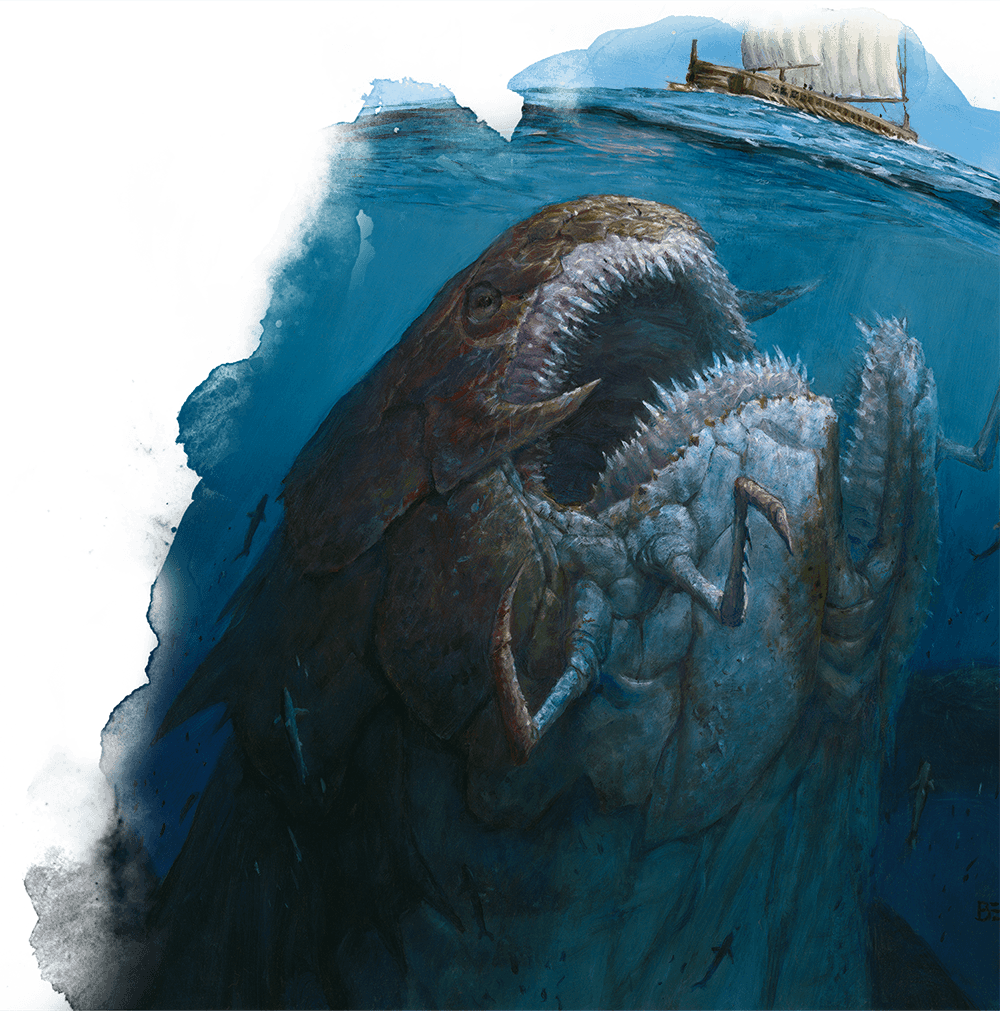
\includegraphics[width=0.5\pdfpagewidth]{03mechanics/img/31friendlyillhevi.png}};
    \end{tikzpicture}

    \newpage

    \begin{DndTable}[width=\linewidth, header=Cold]{cX}
        \textbf{d20} & \textbf{Effect} \\
        1     & Roll damage as normal. \\
        2-3   & The creature may only move half its movement speed on its next turn. \\
        4-6   & The creature has disadvantage on attack rolls until the end of its next turn. \\
        7-8   & The creature’s movement speed is 0 until the end of its next turn. \\
        9-11  & The creature gains vulnerability to bludgeoning damage for a minute. \\
        12-13 & The creature is paralyzed until the end of its next turn. \\
        14-16 & The creature is paralyzed until the end of its next turn.
        If the creature takes damage before the end of its next turn, roll on the minor injury chart. \\
        17-18 & The creature is paralyzed until the end of its next turn and rolls on the minor injury chart. \\
        19    & Roll on the major injury chart. \\
        20    & Roll on the major injury chart, and the creature is paralyzed for the next minute.
        The creature may attempt a Constitution saving throw at the end of each of its turns (DC 15) to end this effect.
        If it fails this saving throw three times it is frozen solid and becomes petrified, but frozen solid rather than turned to stone.
    \end{DndTable}

    \begin{DndTable}[width=\linewidth, header=Fire]{cX}
        \textbf{d20} & \textbf{Effect} \\
        1     & Roll damage as normal. \\
        2-3   & Attack rolls for attacks that deal fire damage have advantage against the creature until the end of its next turn. \\
        4-6   & You burn the creature's hands.
        The creature drops any objects it is holding. \\
        7-8   & The creature is on fire.
        While the creature is on fire it takes 2d4 fire damage at the start of each of its turns.
        The creature can end this condition by dropping prone and using 1 meter of movement to roll on the ground. \\
        9-11  &  \\
        12-13 & The creature is on fire.
        While the creature is on fire it takes 2d6 fire damage at the start of each of its turns.
        The creature can end this condition by dropping prone and using 1 meter of movement to roll on the ground. \\
        14-16 & The creature is charred.
        If the creature has resistance to fire, it loses that resistance.
        If the creature does not have resistance to fire, it gains vulnerability to fire.
        Both of these effects are considered a minor injury. \\
        17-18 & Roll on the minor injury chart.
        Additionally, the creature is on fire.
        While on fire it takes 2d6 fire damage at the start of each of its turns.
        The creature can end this condition by dropping prone and using 1 meter of movement to roll on the ground. \\
        19    & Roll on the major injury chart. \\
        20    & Roll on the major injury chart.
        Additionally, the creature is on fire.
        While the creature is on fire it takes 2d8 fire damage at the start of each of its turns.
        The creature can end this condition by dropping prone and using 1 meter of movement to roll on the ground.
    \end{DndTable}

    \begin{DndTable}[width=\linewidth, header=Force]{cX}
        % TODO: Check back here after done with spells. Dunno if we're keeping Force damage.
        \textbf{d20} & \textbf{Effect} \\
        1     & Roll damage as normal. \\
        2-3   & The creature has disadvantage on saving throws against spells until the end of its next turn. \\
        4-6   & The creature is pushed 3 meters away from you. \\
        7-8   & Spell attack rolls against the creature have advantage until the end of its next turn. \\
        9-11  & The creature is knocked prone. \\
        12-13 & The creature is spellbound until the end of its next turn.
        While spellbound it makes saving throws against spells with disadvantage and spell attack rolls against it have advantage. \\
        14-16 & The creature is spellbound for the next minute.
        While spellbound it makes saving throws against spells with disadvantage and spell attack rolls against it have advantage.
        At the end of each of the creature’s turns it can make an Intelligence saving throw (DC 12) to end this effect. \\
        17-18 & Roll on the minor injury chart.
        Additionally, the creature is spellbound for the next minute.
        While spellbound it makes saving throws against spells with disadvantage and spell attack rolls against it have advantage.
        At the end of each of the creature’s turns it can make an Intelligence saving throw (DC 15) to end this effect. \\
        19    & Roll on the major injury chart. \\
        20    & Roll on the major injury chart.
        Additionally, the creature is spellbound for the next minute.
        While spellbound it makes saving throws against spells with disadvantage and spell attack rolls against it have advantage.
        At the end of each of the creature’s turns it can make an Intelligence saving throw (DC 18) to end this effect.
    \end{DndTable}

    \begin{DndTable}[width=\linewidth, header=Lightning]{cX}
        \textbf{d20} & \textbf{Effect} \\
        1     & Roll damage as normal. \\
        2-3   & The creature cannot use reactions until the end of its next turn. \\
        4-6   & If the creature willingly moves before the start of your next turn, it takes 1d8 lightning damage. \\
        7-8   & You may choose one other creature within 4.5 m. of the victim.
        That creature must succeed on a Dexterity saving throw (DC 12) or take half as much damage. \\
        9-11  & The creature is paralyzed until the start of your next turn. \\
        12-13 & You may choose one other creature within 4.5 m. of the victim.
        That creature must succeed on a Dexterity saving throw (DC 15) or take half as much damage. \\
        14-16 & Roll on the minor injury chart.
        If the creature is wearing metal armor roll on the major injury chart instead. \\
        17-18 & The creature and all creatures within 4.5 m. of it cannot take reactions until the end of their next turn.
        Then roll on the minor injury chart. \\
        19    & Roll on the major injury chart. \\
        20    & All creatures within 4.5 m. of the victim must succeed on a Dexterity saving throw (DC 18) or take half as much damage.
        Then roll on the major injury chart.
    \end{DndTable}

    \begin{DndTable}[width=\linewidth, header=Necrotic]{cX}
        \textbf{d20} & \textbf{Effect} \\
        1     & Roll damage as normal. \\
        2-3   & The creature cannot regain hit points until the end of its next turn. \\
        4-6   & Choose an ability.
        The creature has disadvantage on ability checks made with the chosen ability for a minute. \\
        7-8   & The creature’s maximum hit points are reduced by an amount equal to the damage dealt.
        This lasts until the creature takes a short rest. \\
        9-11  & You heal yourself an amount equal to half of the damage dealt. \\
        12-13 & The creature’s maximum hit points are reduced by an amount equal to the damage dealt.
        This is considered a minor injury. \\
        14-16 & The creature cannot regain hit points for the next minute.
        It may make a Constitution saving throw (DC 15) at the end of each of its turns to end this effect. \\
        17-18 & The creature’s maximum hit points are reduced by an amount equal to the damage dealt.
        This is considered a major injury.
        Then roll on the minor injury chart. \\
        19    & Roll on the major injury chart. \\
        20    & The creature cannot regain hit points for the next minute.
        It may make a Constitution saving throw (DC 18) at the end of each of its turns to end this effect.
        Then roll on the major injury chart.
    \end{DndTable}

    \begin{DndTable}[width=\linewidth, header=Poison]{cX}
        \textbf{d20} & \textbf{Effect} \\
        1     & Roll damage as normal. \\
        2-3   & The creature has disadvantage on its next ability check, attack roll, or saving throw. \\
        4-6   & The creature stinks.
        It has disadvantage on all Charisma checks except Charisma (Intimidation) and Perception checks that rely on smell.
        This lasts until the creature bathes. \\
        7-8   & The creature has disadvantage on all ability checks, attack rolls, and saving throws until the end of its next turn. \\
        9-11  & Any creature in a radius of 2 meters around the target must roll a Constitution saving throw.
        On a failure, they take half the damage dealt. \\
        12-13 & The creature is poisoned for the next minute.
        The creature may attempt a Constitution saving throw at the end of each of its turns (DC 12) to end this effect. \\
        14-16 & The creature is poisoned for the next minute.
        The creature may attempt a Constitution saving throw at the end of each of its turns (DC 15) to end this effect. \\
        17-18 & Roll on the minor injury chart and the creature is poisoned for the next minute.
        The creature may attempt a Constitution saving throw at the end of each of its turns (DC 18) to end this effect. \\
        19    & Roll on the major injury chart. \\
        20    & Roll on the major injury chart, and the creature is poisoned for the next minute.
        The creature may attempt a saving throw at the end of each of its turns (DC 18) to end this effect.
    \end{DndTable}

    \begin{DndTable}[width=\linewidth, header=Psychic]{cX}
        \textbf{d20} & \textbf{Effect} \\
        1     & Roll damage as normal. \\
        2-3   & You control the creature’s movement on its next turn. \\
        4-6   & The creature cannot differentiate friend from foe until the end of its next turn. \\
        7-8   & Attacks against the creature are made with advantage until the start of your next turn. \\
        9-11  & You control the creature’s actions on its next turn. \\
        12-13 & The creature's mind is broken.
        If the creature has resistance to psychic damage, it loses that resistance.
        If the creature does not have resistance to psychic damage, it gains vulnerability to it.
        Both of these effects are considered a minor injury. \\
        14-16 & You control the creature during its next turn. \\
        17-18 & Roll on the Insanity chart with disadvantage. \\
        19    & Roll on the Insanity chart. \\
        20    & Roll on the Insanity chart with advantage.
    \end{DndTable}

    \begin{DndTable}[width=\linewidth, header=Radiant]{cX}
        \textbf{d20} & \textbf{Effect} \\
        1     & Roll damage as normal. \\
        2-3   & The has disadvantage on any Perception checks that rely on sight.
        This is considered a minor injury. \\
        4-6   & The creature's attack rolls are made with disadvantage. \\
        7-8   & The creature is blinded until the end of its next turn. \\
        9-11  & The creature is blinded for a minute.
        It can make a Constitution saving throw (DC 12) at the end of each of its turns to end this effect. \\
        12-13 & The creature glows for the next minute.
        While glowing it produces bright light up 2 meters and dim light up to 6 meters and all successful attacks against the creature deal an additional 1 radiant damage. \\
        14-16 & The creature is frightened of you for the next minute.
        It can make a Wisdom saving throw (DC 15) at the end of each of its turns to end this effect. \\
        17-18 & Roll on the minor injury chart.
        Additionally, the creature glows for the next minute.
        While glowing it produces bright light up 2 meters and dim light up to 6 meters and all successful attacks against the creature deal an additional 1d4 radiant damage. \\
        19    & Roll on the major injury chart. \\
        20    & Roll on the major injury chart.
        Additionally, the creature glows for the next minute.
        While glowing it produces bright light up 2 meters and dim light up to 6 meters and all successful attacks against the creature deal an additional 1d6 radiant damage.
    \end{DndTable}

    \pagebreak~
    \begin{tikzpicture}[remember picture,overlay]
        \node[anchor=north, yshift=0.10cm] at (current page.north) {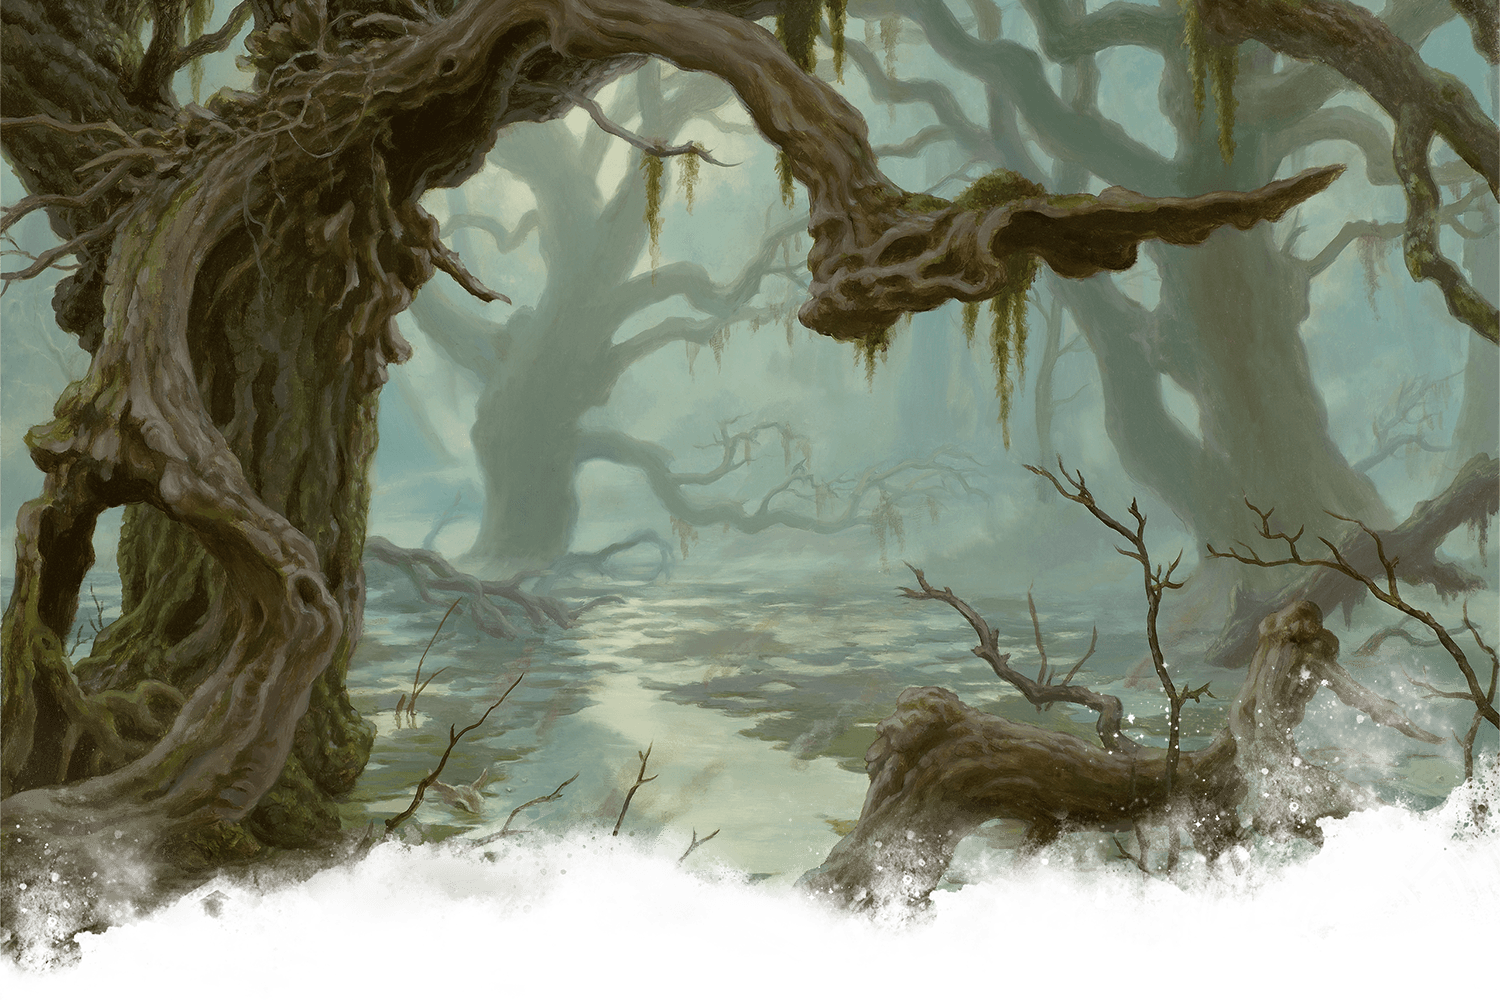
\includegraphics[width=\pdfpagewidth]{03mechanics/img/31arastas_domain.png}};
    \end{tikzpicture}

    \vspace{12.0cm}

    \begin{DndTable}[width=\linewidth, header=Thunder]{cX}
        \textbf{d20} & \textbf{Effect} \\
        1     & Roll damage as normal. \\
        2-3   & The creature has disadvantage on any Perception checks that rely on hearing.
        This is considered a minor injury. \\
        4-6   & The creature is deafened until the end of its next turn. \\
        7-8   & The creature is confused until the end of its next turn.
        While confused, the creature moves in a random direction determined by the DM. \\
        9-11  & The creature is deafened for one minute. \\
        12-13 & The creature is stunned until the start of its next turn and is deafened for one minute. \\
        14-16 & The creature is deafened permanently.
        This is considered a major injury. \\
        17-18 & The creature is stunned until the end of its next turn and is deafened for one minute.
        Then roll on the minor injury chart. \\
        19    & Roll on the major injury chart. \\
        20    & The creature is stunned until the end of its next round and is deafened for one minute.
        Then roll on the major injury chart.
    \end{DndTable}
